\pdfoutput=1
\documentclass[11pt]{article}

% Remove the "review" option to generate the final version.
\usepackage{emnlp2021}
\usepackage{float} 
\usepackage{amssymb}
\usepackage{amsmath}
\usepackage{times}
\usepackage{latexsym}
\usepackage[T1]{fontenc}
\usepackage[utf8]{inputenc}
\usepackage{microtype}
\usepackage{graphicx}
\usepackage[english]{babel}
\usepackage{xcolor}
\usepackage{array}
\usepackage{multirow}
\usepackage{bigdelim}
\usepackage{booktabs}
\newcommand{\R}{\mathbb{R}}
\newcolumntype{P}[1]{>{\centering\arraybackslash}p{#1}}
\title{Matching The Statements: A Simple and Accurate Model \\ for Key Point Analysis}

\author{Viet Hoang Phan \hspace*{3mm} Tien Long Nguyen \hspace*{3mm} Duc Long Nguyen \hspace*{3mm} Ngoc Khanh Doan\\
School of Information and Communication Technology \\
Hanoi University of Science and Technology\\
\texttt{\{hoang.pv180086, long.nt180129, long.nd183583,}\\
\texttt{khanh.dn180110\}@sis.hust.edu.vn}
}

\begin{document}
\maketitle

\begin{figure*}[ht!]
\centering
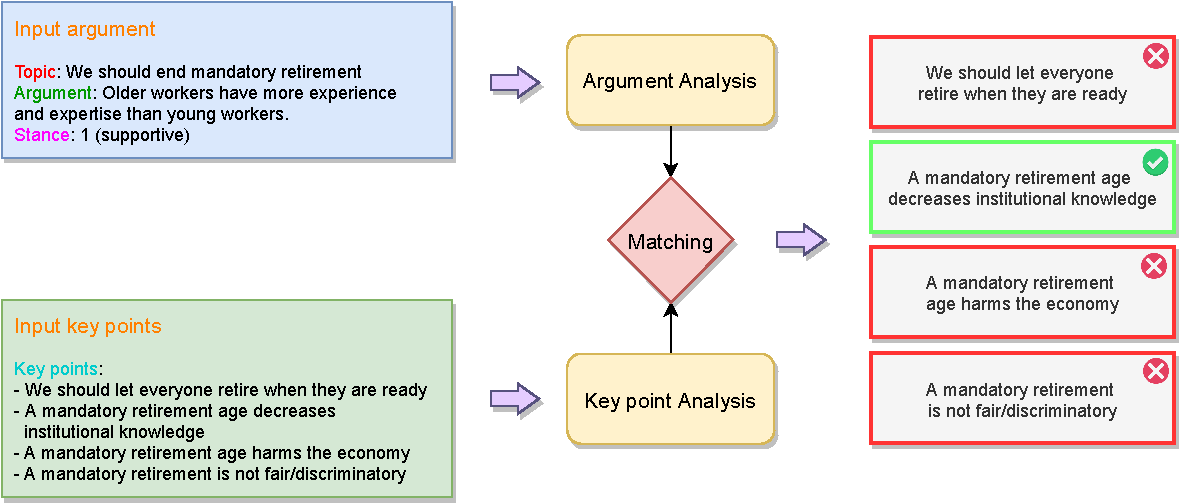
\includegraphics[scale=0.74]{figures/KPA-workflow.pdf}
\caption{Overview of the Key Point Matching workflow in the Quantitative Summarization – Key Point Analysis Shared Task Track 1. From the information retrieval perspective, this task is to identify the most salient point that reinforces a given query.}
\label{fig:workflow}
\end{figure*}


\begin{abstract}
Key Point Analysis (KPA) is one of the most essential tasks in building an Opinion Summarization system, which is capable of generating key points for a collection of arguments toward a particular topic. Furthermore, KPA allows quantifying the coverage of each summary by counting its matched arguments. With the aim of creating high-quality summaries, it is necessary to have an in-depth understanding of each individual argument as well as its universal semantic in a specified context. In this paper, we introduce a promising model, named Matching the Statements (MTS) that incorporates the discussed topic information into arguments/key points comprehension to fully understand their meanings, thus accurately performing ranking and retrieving best-match key points for an input argument. Our approach\footnote{The code is available at: \url{https://github.com/VietHoang1512/KPA}} has achieved the $4^{th}$ place in Track 1 of the Quantitative Summarization – Key Point Analysis Shared Task by IBM, yielding a competitive performance of $0.8956\:(3^{rd})$ and $0.9632\:(7^{th})$ strict and relaxed mean Average Precision, respectively.
\end{abstract}

\section{Introduction}
\label{sec:intro}

Prior work in Opinion Summarization often followed the extractive strategy, which identifies the most representative pieces of information from the source text and copies them verbatim to serve as summaries \citep{angelidis-lapata-2018-summarizing, brazinskas2019unsupervised}. Abstractive summarization is a less popular strategy compared to the previous one yet offers more coherent output texts. Approaches governed by this vein could generate new phrases, sentences or even paragraphs that may not appear in the input documents \citep{ganesan-etal-2010-opinosis, isonuma2021unsupervised}. Both extractive and abstractive methods are the straightforward applications of multi-document summarization \citep{liu2018generating, fabbri-etal-2019-multi}, which has been an emerging research domain of natural language processing in recent years.

As is well known, in traditional multi-document summarization methods, the role of an individual or a subset of key points among the summaries is often neglected. To be more specific, \citet{bar-haim-etal-2020-arguments} posed a question regarding the summarized ability of a small group of key points, and to some extent answered that question on their own by developing baseline models that could produce a concise bullet-like summary for the crowd-contributed arguments.
With a pre-defined list of summaries, this task is known as Key Point Matching (KPM). Figure \ref{fig:workflow} provides a simple illustration of the KPM problem, where the most relevant key points are retrieved for each given argument within a certain topic (i.e. context).

Inspired by the previous work that studied the problem of learning sentence representation \citep{cer2018universal, reimers-gurevych-2019-sentence} and semantic similarity \citep{yan2021consert}, we propose Matching The Statements (MTS), which further takes the topic information into account and effectively utilizes such proper features to learn a high performance unified model. Our approach has benefited from the recent developments of pre-trained language models such as BERT \citep{devlin2018bert}, ALBERT \citep{lan2019albert} or RoBERTa \citep{liu2019roberta}.

Our contributions in this paper could be depicted as follows:
\begin{itemize}
    \item Firstly, we design a simple yet efficient network architecture to fuse the context into sentence-level representations. Instead of letting the model infer the implicit reasoning structure, we provide our model with the information on whether an argument or key point (which are collectively referred to as statements in the remainder of this paper) supports its main topic or not.
    \item Secondly, our method adopts the pseudo-labels mechanism \citep{ge2020mutual, zhang2021refining}, where we label arguments that belong to the same key point (and the key point itself) by the same index. The goal is to learn an embedding space in which the embedded vectors of mutual supportive statement pairs (i.e. having the same label) are pulled closer whereas unrelated ones are pushed apart. 
    \item Finally, we validate the proposed MTS on the ArgKP-2021 \citep{bar-haim-etal-2020-arguments} dataset in a variety of protocols. Extensive experiment results show that our proposed method strongly outperforms other baselines without using external data, thus becoming a potential method for the Key Point Matching problem.
\end{itemize}

The rest of this paper is organized in the following way: Section \ref{sec:related-work} briefly reviews the related work, while section \ref{sec:problem} formulates the KPM problem. Next, we describe our methodology in section \ref{sec:method}, followed by the experimental results in section \ref{sec:experiment}. Finally, section \ref{sec:conclusion} will conclude our work and discuss future directions for further improvements.



\begin{figure*}[ht!]
\centering
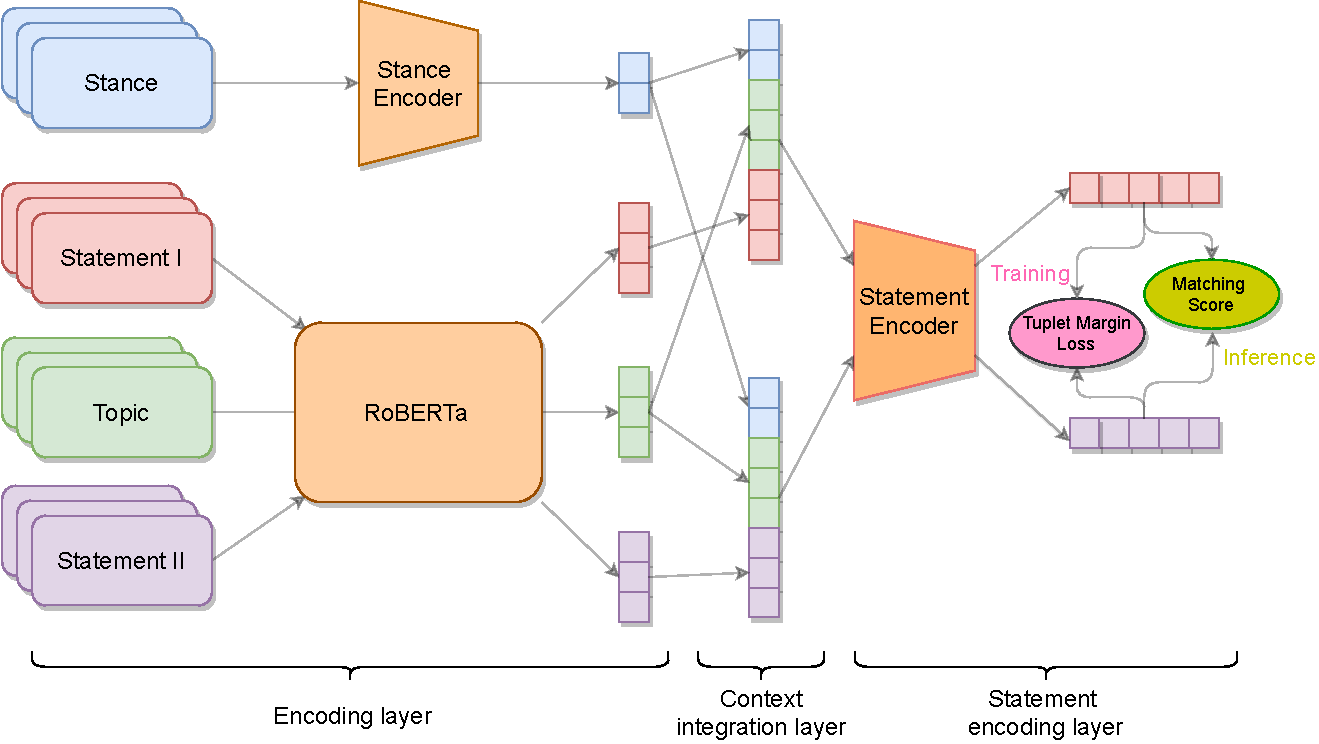
\includegraphics[scale=0.6]{figures/KPA-model.pdf}
\caption{The overall design of our Matching The Statements architecture.}
\label{fig:model}
\end{figure*}

\section{Related Work}
\label{sec:related-work}
A standard approach for key points and arguments analysis is properly extracting their meaningful semantics. Our model stems from recent literatures that are based on siamese neural networks \citep{reimers-gurevych-2019-sentence, gao2021simcse} to measure the semantic similarity between documents. Even though, MTS has its own unique characteristics to incorporate context information.
\subsection{Sentence Embeddings} 
The representation of sentences in a fixed-dimensional vector space plays a crucial role in enhancing a model's performance on downstream tasks. Early methods relied on static word embeddings \citep{pennington-etal-2014-glove, bojanowski2017enriching}, which encoded a sentence by directly averaging its word vectors or employing recurrent neural network (RNN) encoders \citep{conneau-etal-2017-supervised} and taking the pooled output from the hidden units. Despite the fact that these methods can leverage both syntactic and semantic features, they often fail to retain the contextual information or suffer from slow training (due to the sequential nature of RNNs). 

That is where BERT \cite{devlin2018bert} as well as its variants come in and dominate the modern NLP research. Training these architectures can exploit the parallel computational capacity of GPUs/TPUs hardware accelerators. In SBERT, \citet{reimers-gurevych-2019-sentence} proposed a sentence embedding method via fine-tuning BERT models on natural language inference (NLI) datasets. More recent studies in learning sentence representation followed the contrastive learning paradigm and achieved state-of-the-art performance on numerous of benchmark tasks \citep{liao2021sentence, yan2021consert}.

\subsection{Semantic matching} 

Semantic matching is a long-standing problem and has a wide range of applications, such as: question-answering \citep{yang-etal-2015-wikiqa}, text summarization \citep{zhong-etal-2020-extractive} and especially, information retrieval \citep{huang2013learning, guo2016deep}. \citet{jiang2019semantic} introduced a hierarchical recurrent neural network that could capture long-term dependency and synthesize information from different granularities (i.e. words, sentences or paragraphs). Similarly, \citet{yang2020beyond} replaced the RNN backbones with transformer-based models and modified self-attention architectures to adapt with long document inputs. 

However, most of the existing work focuses only on assessing the similarity between pairs of sentences without paying attention to their context - which can help the reader to get an overview of the discussed topic. Recently, the ArgKP-2021 dataset has been published by \citet{bar-haim-etal-2020-arguments}, which consists of annotations about whether two statements and their stances towards a specific topic match or not. The next sections will provide an overview of this dataset and how our model is applicable in the Quantitative Summarization – Key Point Analysis Shared Task \footnote{\url{https://2021.argmining.org/shared_task_ibm.html}}.

\section{Problem definition}
\label{sec:problem}
In this shared task, we are provided with a dataset consisting of 28 different topics. Each topic contains a set of associated arguments and key points in the form of matching (with label 1) or non-matching (with label 0) pairs. The stances of these statements (whether a claim agrees or disagrees with its topic) are also exposed, we further evaluate the impact of this information in section \ref{sec:stance}.

In short, the Key Point Matching problem is formulated as follows: Given a controversial topic $T$ with a list of $m$ arguments and $n$ key points $A_1, A_2, \dots, A_m ;\;K_1, K_2, \dots, K_n$, along with their corresponding stances $S_1, S_2, \dots, S_{m+n} \; (S_i \in \{-1, 1\})$, which imply the attack or support relationships against the topic, our task is to rank key points that have the same stance with an input argument by the matching score. This priority is dependent on both the topic and the semantic of statements.




\section{Methodology}
\label{sec:method}

The proposed MTS architecture is graphically shown in figure \ref{fig:model}. It takes four separate inputs: (i) discussed topic, (ii) first statement, (iii) second statement, and (iv) their stance toward the topic. The final output is the similarity score of the fed in statements with respect to the main context. In the remainder of this section, we would like to describe three main components of MTS: encoding, context integration and statement encoding layers.

\subsection{Data preparation}
\label{sec:prepare}
We observe that a small percentage of the arguments ($4.71\%$) belong to two or more key points, while the rest are matched with at most one. For that reason, a straightforward idea is gathering arguments, which belong to the same key point, and label the clusters in order. In other words, each cluster is represented by a key point $K_i$, contains $K_i$ and its matching arguments. Our clustering technique results in the fact that there are a small number of arguments that belong to multiple clusters. Arguments that do not match any of the key points are grouped into the NON-MATCH set.

Intuitively, if two different arguments support the same key point, they tend to convey similar meanings and should be considered as a matching pair of statements. Conversely, statements from different clusters are considered non-match in our approach. This pseudo-label method thus utilizes the similar semantic of within-cluster documents and enhances the model robustness. In the remainder of this paper, those arguments that come from the same cluster are referred to as positive pairs, otherwise, they are negative pairs.

During training, we use each key point and its matching/non-matching arguments (based on the annotation in the ArgKP-2021 dataset) in a mini-batch. Moreover, we also sample a small proportion of the NON-MATCH arguments and merge them into the mini-batch. Specifically, all the NON-MATCH arguments are considered to come from different and novel clusters. Because the definition of positive/negative statement pairs is well-defined, we can easily compute the loss in each mini-batch with a usual metric learning loss \citep{chopra2005learning, yu2019deep}.% A contrastive loss will be employed to enclose the distance between intra-cluster samples as well as to enlarge the distance between that of inter-cluster ones.

\subsection{Encoding layer}

We first extract the contextualized representation for textual inputs using the RoBERTa \citep{liu2019roberta} model. We adopt a canonical method \citep{sun2019fine} to achieve the final embedding of a given input, which is concatenating the last four hidden states of the [CLS] token. These embeddings are fed into the context integration layer as an aggregate representation for topics, arguments and key points. For example, a statement vector at this point is denoted as \footnote{For a consistent notation, statements and stances are denoted by uppercase letters: $X$ and $S$}: 
\begin{align*}
\mathbf{h}^X = [\:h^X_1, h^X_2, \dots, h^X_{4\times768}\:]\;\; (h^X_i \in \R ) \\
    = [\:h^X_1, h^X_2, \dots, h^X_{3072}\:] \hspace*{20mm}
\end{align*}
with 768 is the number of hidden layers produced by the RoBERTa-base model. 

For the stance encoding, we employ a fully-connected network with no activation function to map the scalar input to a $N$-dimensional vector space. The representation of each topic, statement and stance are denoted as $\mathbf{h}^T, \mathbf{h}^X$ and $\mathbf{h}^S$, respectively.

\subsection{Context integration layer}

After using the RoBERTa backbone and a shallow neural network to extract the embeddings acquired from multiple inputs, we conduct a simple concatenation with the aim of incorporating the topic (i.e. context) and stance information into its argument/key point representations. After this step, the obtained vector for each statement is ($[;]$ notation indicates the concatenation operator):
\begin{align*}
\mathbf{v}^X = [\mathbf{h}^S; \mathbf{h}^T; \mathbf{h}^X] 
\end{align*}
where $\mathbf{v}^X \in \R^{N+2\times3072}$

% Since these
\subsection{Statement encoding layer}
The statement encoding component has another fully-connected network on top of the context integration layer to get the final $D$-dimensional embeddings for key points or arguments:
\begin{align*}
\mathbf{e}^X = \mathbf{v}^X\:\mathbf{W} + \mathbf{b}
\end{align*}
where $\mathbf{W} \in \R^{ (N+6144) \times D}$ and $ \mathbf{b} \in \R^{D}$ are the weight and bias parameters.

Concretely, training our model is equivalent to learning a function $f(S,T,X)$ that maps the similar statements onto close points and dissimilar ones onto distant points in $\R^{ (N+6144) \times D}$.

\subsection{Training}
\label{sec:training}
In each iteration, we consider each input statement from the incoming mini-batch as an anchor document and sample positive/negative documents from within/inter clusters. For calculating the matching score between two statements, we compute the cosine distance of their embeddings:
\begin{align}
\mathcal{D}_{\mathrm{cosine}}(\mathbf{e}^{X_1}, \mathbf{e}^{X_2}) =
1 - \mathrm{cos}(\mathbf{e}^{X_1}, \mathbf{e}^{X_2}) \label{eq:cosine}\\
= 1 - \frac{{\mathbf{e}^{X_1}}^T \mathbf{e}^{X_2}}
{||\mathbf{e}^{X_1}||_2 \: ||\mathbf{e}^{X_2}||_2} \nonumber
\end{align}

Empirical results show that cosine distance yields the best performance compared to Manhattan distance ($||\mathbf{e}^{X_1} - \mathbf{e}^{X_2}||_1$) and Euclidean distance ($||\mathbf{e}^{X_1} - \mathbf{e}^{X_2}||_2$). Hence, we use cosine as the default distance metric throughout our experiments. We also revisit several loss functions, such as contrastive loss \citep{chopra2005learning}, triplet loss \citep{dong2018triplet} and tuplet margin loss \citep{yu2019deep}. Unlike previous work, \citet{yu2019deep} use another distance metric, which will be described below.

Assume that a mini-batch consists of $k+1$ samples $\{X_a, X_p, X_{n_{1}},X_{n_{2}}, \dots, X_{n_{k-1}}\}$, which satisfies the tuplet constraint: $X_p$ is a positive statement whereas $X_{n_i}$ are $X_a$'s negative statements w.r.t $X_a$. Mathematically, the tuplet margin loss function is defined as:
\begin{align*}
\mathcal{L}_{\text{tuplet}} = \log(1 + \sum_{i=1}^{k-1} 
\mathrm{e}^{s(\mathrm{cos}\:\theta_{an_i} - \mathrm{cos}\:(\theta_{ap}-\beta))} )
\end{align*}
where  $\theta_{ap}$ is the angle between $e^{X_a}$ and $e^{X_p}$;\; $\theta_{an_i}$ is the angle between $e^{X_a}$ and $e^{X_{n_{i}}}$. $\beta$ is the margin hyper-parameter, which imposes the distance between negative pair to be larger than $\beta$. Finally, $s$ acts like a scaling factor.

Additionally, \citet{yu2019deep} also introduced the intra-pair variance loss, which was theoretically proven to mitigate the intra-pair variation and improve the generalizability. In MTS, we use a weighted combination of both tuplet margin and intra-pair variance as our loss function. The formulation of the latter one is:
\begin{align*}
\mathcal{L}_{pos} = \mathbb{E}[(1-\epsilon)\:\mathbb{E}[\mathrm{cos}\:\theta_{ap}] - \mathrm{cos}\:\theta_{ap}]^2_+ \\
\mathcal{L}_{neg} = \mathbb{E}[\mathrm{cos}\:\theta_{an} - (1+\epsilon)\:\mathbb{E}[\mathrm{cos}\:\theta_{an}]^2_+ \\
\mathcal{L}_{\mathrm{intra-pair}} = \mathcal{L}_{pos} + \mathcal{L}_{neg} \hspace*{10mm}
\end{align*}
where $[\cdot]_+ = \mathrm{max}(0, \cdot )$.

As pointed out by \citet{hermans2017defense, wu2017sampling}, training these siamese neural networks raises a couple of issues regarding easy/uninformative examples bias. In fact, if we keep feeding random pairs, more easy ones are included and prevent models from training. Hence, a hard mining strategy becomes crucial for avoiding learning from such redundant pairs. In MTS, we adapt the multi-similarity mining from \citet{wang2019multi}, which identifies a sample's hard pairs using its neighbors.

Given a pre-defined threshold $\epsilon$, we select the negative pairs if they have the cosine similarity greater than the hardest positive pair, minus $\epsilon$. For instance, let $X_a$ be a statement, which has its positive and negative sets of statements denoted by $\mathcal{P}_{X_a}$ and $\mathcal{N}_{X_a}$, respectively.
A negative pair of statements $\{X_a, X_n\}$ is chosen if:
\begin{align*}
\mathrm{cosine}(\mathbf{e}^{X_a}, \mathbf{e}^{X_n}) \geq \underset{X_i\in \mathcal{P}_{X_a}}\min \mathrm{cosine}(\mathbf{e}^{X_a}, \mathbf{e}^{X_i})-\epsilon
\end{align*}
Such pairs are referred to as hard negative pairs, we carry out a similar process to form hard positive pairs. If a positive pair $\{X_a, X_p\}$ is selected, then:
\begin{align*}
\mathrm{cosine}(\mathbf{e}^{X_a}, \mathbf{e}^{X_p}) \leq \underset{X_i\in \mathcal{N}_{X_a}}{\max}   \mathrm{cosine}(\mathbf{e}^{X_a}, \mathbf{e}^{X_i})+\epsilon
\end{align*}
\subsection{Inference}
At inference time, we pair up the arguments and key points that debate on a topic under the same stance. Afterward, we compute the matching score based on the angle between their embeddings. For instance, an argument $A$ and key point $K$ will have a matching score of:
\begin{align*}
% \mathbf{u}^A = \frac{\mathbf{e}^A}{||\mathbf{e}^A||_2} \; \; \;; \; \; \;
% \mathbf{u}^K = \frac{\mathbf{e}^K}{||\mathbf{e}^K||_2} \\
% \vspace*{2mm}\mathrm{score}(\mathbf{e}^A, \mathbf{e}^K) = \frac{\pi - \angle\:(\mathbf{u}^A, \mathbf{u}^K)}{\pi-\beta}\\
\mathrm{score}(\mathbf{e}^A, \mathbf{e}^K) = 1 - \mathcal{D}_{\mathrm{cosine}}(\mathbf{e}^A, \mathbf{e}^K)\\
= \mathrm{cos}(\mathbf{e}^A, \mathbf{e}^K)\hspace*{12.5mm}
\end{align*}

The right-hand side function squashes the score into the probability interval of $[0,1)$ and compatible with the presented loss function in section \ref{sec:training}.

\section{Experiment}
\label{sec:experiment}


To verify the effectiveness of the Matching The Statements model, we conduct extensive experiments on the ArgKP-2021 \citep{bar-haim-etal-2020-arguments} dataset and compare the performance of MTS against baselines. 

\subsection{ArgKP-2021 Dataset}

ArgKP-2021 \citep{bar-haim-etal-2020-arguments}, the data set used in the Quantitative Summarization – Key Point Analysis Shared Task, is split into training and development sets with the ratio of $24:4$. The training set is composed of 5583 arguments and 207 key points while those figures in the development set are 932 and 36. Each argument could be matched to one or more key points, yet the latter ones account for a small proportion of the data, as stated in section \ref{sec:prepare}. The texts presented in ArgKP-2021 are relatively short, with approximately $18.22 \pm 7.76$ by words or $108.20 \pm 43.51$ by characters.

\subsection{Evaluation protocol}

For evaluation, only the most likely key point is chosen for each argument based on the predicted scores. These pairs are then sorted by their matching scores in descending order, and only the first half of them are included in the assessment. According to \citet{kpa-2021-overview}, there are two metrics used in Track 1, namely relaxed and strict mean Average Precision (mAP):
\begin{align*}
\mathbf{Precision} = \frac{\mathrm{True\:Positive}}
{\mathrm{True\:Positive} + \mathrm{False\:Positive}}
\end{align*}

Since there are some argument-key point pairs in the ArgKP-2021 dataset that have indecisive annotations (i.e. their label is neither matched nor non-matched): in the relaxed mAP evaluation, these pairs are considered as matched whereas strict mAP treats them as non-matched pairs.

\begin{figure}[ht]
\centering
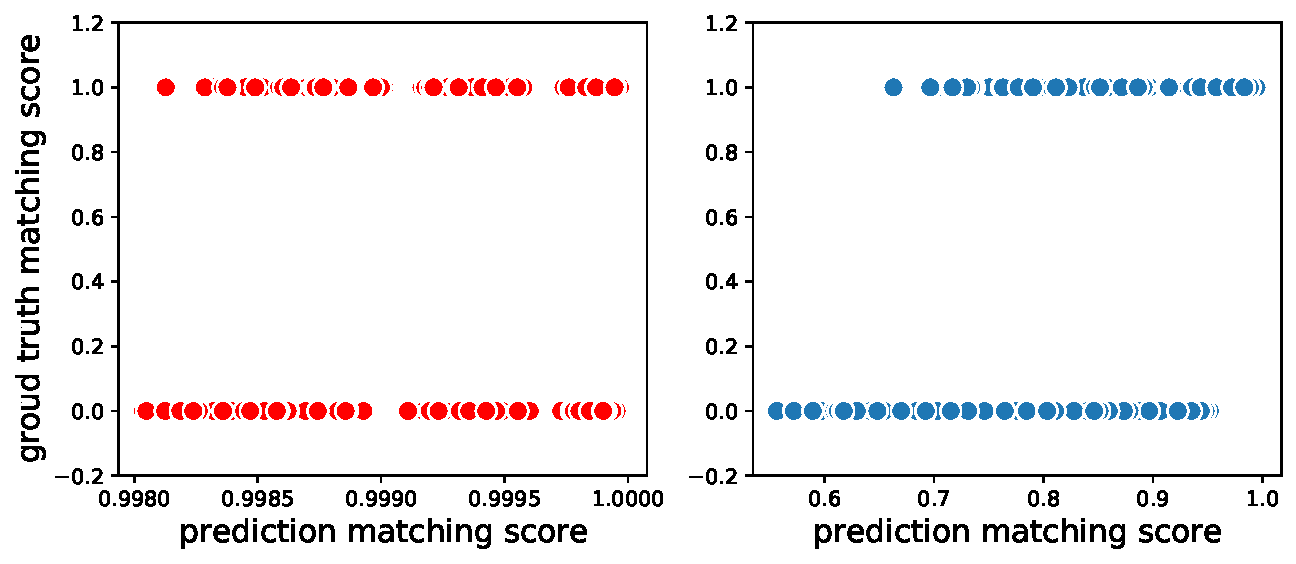
\includegraphics[scale=0.35]{figures/before-after.pdf}
\caption{Statement representation before (left) and after (right) training.}
\label{fig:before-after}
\end{figure}

\subsection{Embeddings quality}

Figure \ref{fig:before-after} depicts the qualitative representation learning result of MTS before and after training. In the beginning, the similarity scores between matched/non-match key point-argument pairs are extremely high ($\approx0.999$). That means, almost all the statements are projected into a small region of the embedding space, and it is difficult to derive a cut-off threshold to get rid of the non-matching pairs.

Therefore, the mean Average Precision scores when we directly use the untrained model with RoBERTa backbone are relatively low. Though, our training procedure improves the model's distinguishability and reduces the collapsed representation phenomenon. Indeed, the similarity scores at this point are stretched out and the mAP scores significantly increase ($\text{strict\:mAP}\;0.45\to0.84;\\ \text{relaxed\:mAP}\:0.62\to0.94$).

\begin{figure}[t]
\centering
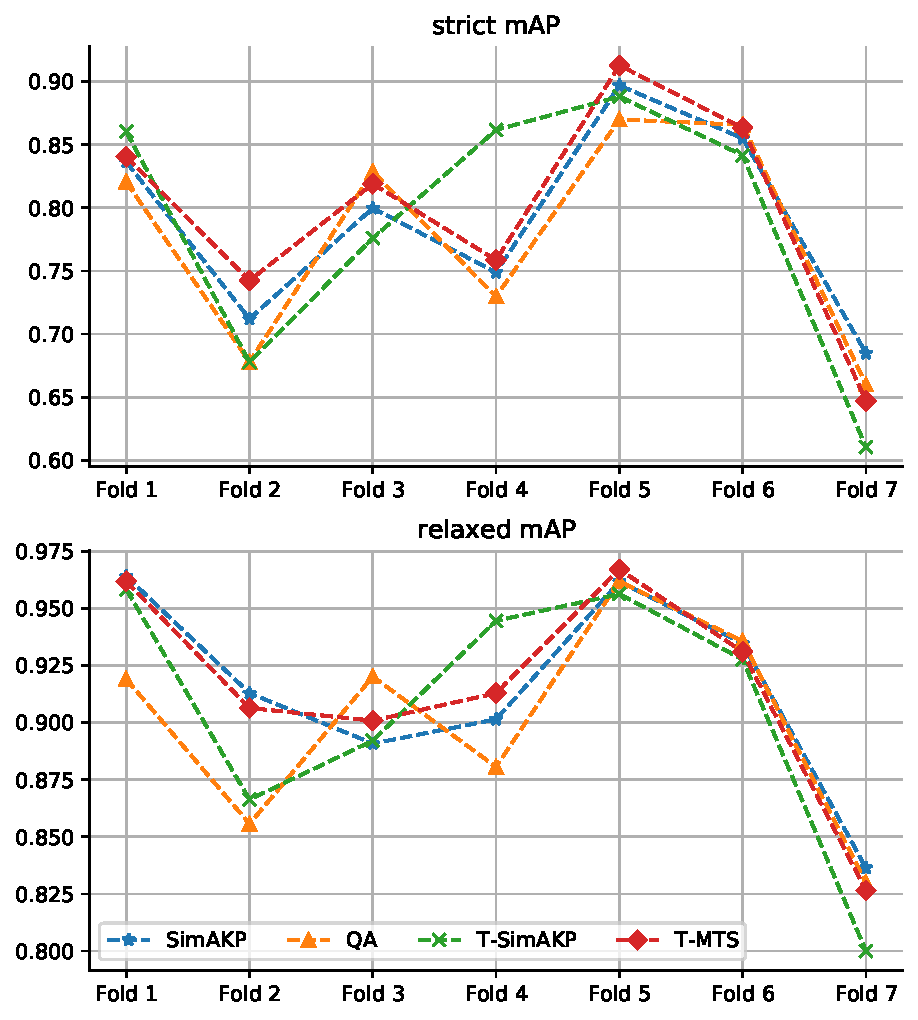
\includegraphics[scale=0.49]{figures/7-folds.pdf}
\caption{Mean Average Precision scores over 7 folds. The "T-" prefix denotes the models that use triplet loss \citep{dong2018triplet} while the rest are trained with the contrastive loss \citep{chopra2005learning}.}
\label{fig:7-folds}
\end{figure}

\subsection{Baselines}

For performance benchmarking, we implement two different baselines and their variations, namely Simple Argument-Key point matching (SimAKP) and Question Answering-liked Argument-Key point matching (QA) models. We construct a sampling strategy in an online manner: in each mini-batch, we select the hardest positive/negative pairs according to the method discussed in Section \ref{sec:training} to compute the loss.

\textbf{Simple Argument-Key point matching:} The architecture of SimAKP is the same as MTS with the main difference in the data preparation. Instead of clustering similar statements, SimAKP simply performs pair-wise classification on the ArgKP-2021 dataset. Equivalently, each input to the SimAKP model consists of an argument-key point pair. This approach will not make use of the analogous nature of these claims that matched with the same key point.

\textbf{Question Answering-liked Argument-Key point matching:} Inspired by the Question Answering, we format the arguments and key points fed to the RoBERTa model in order to incorporate the context into statements as below:

\hspace*{3mm}[CLS] Topic [SEP] [SEP] Statement [SEP]

\hspace*{3mm}[CLS] Topic  [SEP] [SEP] Key point [SEP]

where [CLS] and [SEP] are two special tokens.

In particular, obtained outputs of RoBERTa model with the above inputs are then concatenated with the stance representations to produce a tensor with shape $(\mathrm{batch\:size}, N+3072)$, which is fed to a fully connected layer to embed the semantic meaning of each individual statement.
\subsection{Results}

To facilitate evaluation, we set up a 7-fold cross-validation, each contains 24 topics for training and 4 topics for development. The train-dev split in Track 1 of Quantitative Summarization – Key Point Analysis Shared Task is replicated in fold 1.

As can be seen in Figure \ref{fig:7-folds}, we observe that our proposed MTS (we use triplet loss for a fair comparison) consistently outperforms other baselines in both mAP scores (higher is better). It achieved competitive scores on all splits, except fold 7. The reason is that the number of labeled argument-key point pairs of the development set in this part is the smallest among 7 folds, and there are substantial drops in terms of performance for all baselines.
\begin{table}[ht]
\centering
\begin{tabular}{|c|c|c|}
\hline
\textbf{Model} & \textbf{strict mAP} & \textbf{relaxed mAP}\\
\hline\hline
    SimAKP 
    & $0.790 \pm 0.072$ & $0.914 \pm 0.041$   \\
    \begin{tabular}{@{}c@{}}SimAKP \\\noindent w.o mining\end{tabular} 
    & $0.783 \pm 0.074$ & $0.917 \pm 0.037$   \\
    T-SimAKP 
    & $0.788 \pm 0.098$ & $0.906 \pm 0.054$   \\
    \begin{tabular}{@{}c@{}}T-SimAKP \\\noindent w.o mining\end{tabular} 
    & $0.782 \pm 0.101$ & $0.901 \pm 0.076$   \\
\hline
\end{tabular}
\caption{\label{tab:hard-mining}
The effect of hard sample mining in baselines.
}
\end{table}

We also examine the impact of hard negative mining in Table \ref{tab:hard-mining}, the baselines are compared against themselves when using the hard mining strategy (i.e. avoid learning the embeddings of trivial samples). With the employment of hard mining, there is an improvement in performance for most baselines. Except for a small decrease in terms of relaxed mAP in SimAKP, both contrastive and triplet loss Simple Argument-Key point matching models have an average increase of 0.005\% in mAP scores.

\subsection{Differential Analysis}
To provide insight analysis in the setting of Matching The Statements, we therefore create four different setups: original MTS, MTS with batch normalization \citep{ioffe2015batch} immediately after context integration layer, MTS without mining strategy, and triplet-loss MTS. Although tuplet margin loss has an up/down weighting hard/easy samples mechanism, we find that MTS with multi-similarity mining \citep{wang2019multi} performed best during the exploratory phase. 

\begin{figure}[h]
\centering
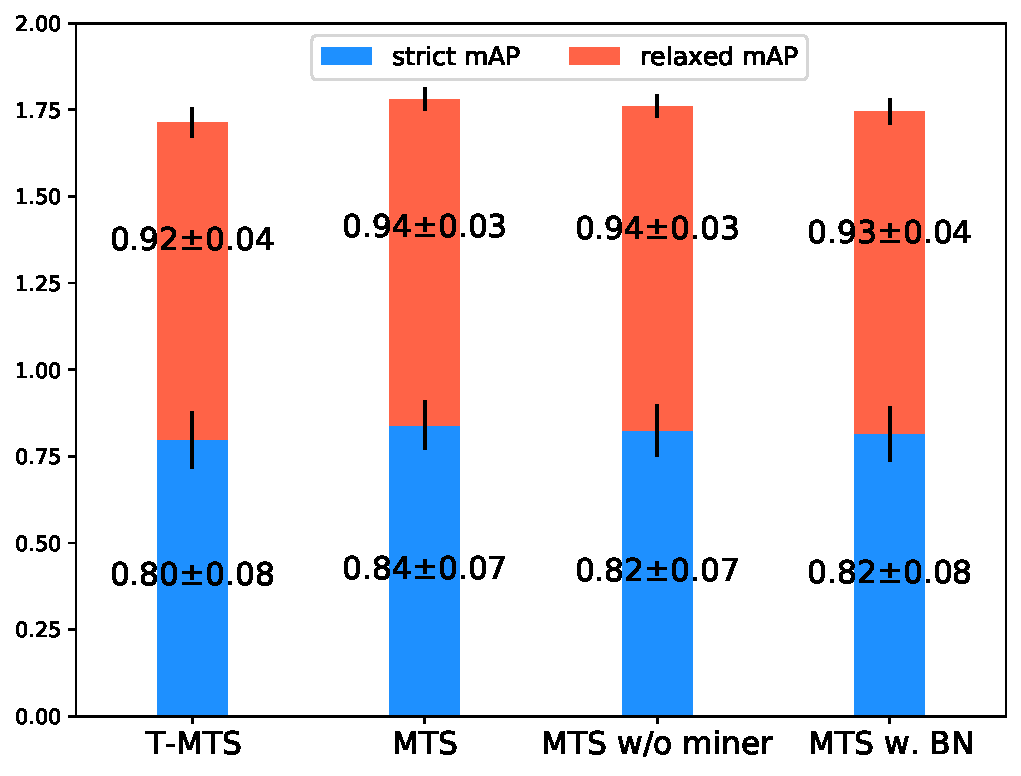
\includegraphics[scale=0.44]{figures/modification.pdf}
\caption{Switching off different setups shows that each component of the original MTS's setting contributes to its performance.}
\label{fig:modification}
\end{figure}

Figure \ref{fig:modification} summarizes the average score for all setups. Overall, MTS performs similarly or better than its variants (without multi-similarity mining or adding a batch normalization layer). Replacing triplet loss with tuplet margin loss helps to boost both strict mAP and relaxed mAP by 0.2. Eventually, in an attempt to produce a consistent and accurate prediction on the test dataset, an ensemble of 4/7 best models from splits was used for final submission. As shown in Table \ref{tab:leaderboard}, among the performances of the top-10 team, our proposed model achieved the third position in terms of strict mAP, $7^{th}$ position in relaxed mAP and $4^{th}$ overall.
\begin{table}[ht]
\centering
\begin{tabular}{|P{3mm}|P{22mm}|P{17mm}|P{17mm}|}
\hline
\textbf{\#} & \textbf{Team} & \textbf{strict mAP} & \textbf{relaxed mAP}\\
\hline\hline
    $1$ & mspl & $0.908\:(2)$ & $0.972\:(3)$   \\
    $2$ & heinrichreimer & $0.912\:(1)$ & $0.967\:(5)$   \\
    $3$ & vund & $0.878\:(4)$ & $0.968\:(4)$   \\
    $\mathbf{4}$ & \textbf{HKL\:(ours)} & $\mathbf{0.896\:(3)}$ & $\mathbf{0.963\:(7)}$   \\
    $5$ & sohanpatnaik & $0.872\:(5)$ & $0.966\:(6)$   \\
    $6$ & fengdoudou & $0.853\:(10)$ & $0.98\:(2)$   \\
    $7$ & mozhiwen & $0.833\:(12)$ & $0.985\:(1)$   \\
    $8$ & Fibelkorn & $0.869\:(6$ & $0.952\:(10)$   \\
    $8$ & emanuele.c & $0.868\:(7)$ & $0.956\:(9)$   \\
    $10$ & niksss & $0.858\:(8)$ & $0.95\:(11)$   \\
\hline
\end{tabular}
\caption{\label{tab:leaderboard}
Leaderboard of the Track 1 Quantitative Summarization – Key Point Analysis.
}
\end{table}
\subsubsection{BERT embeddings}
\label{sec:bert_emb}

\begin{table*}[t]
\centering
\begin{tabular}{|c|c|c|c|}
\hline
\textbf{Embedding} & \textbf{strict mAP} & \textbf{relaxed mAP} & \textbf{\#Param}\\
\hline\hline
    {Sum all tokens}
    & $0.834 \pm 0.065$ & $0.938 \pm0.037$  & \multirow{3}*{$125$M}\\
    {Mean all tokens}
    & $0.796 \pm 0.068$ & $0.916 \pm0.034$  & \\
    {[CLS] last hidden layer}
    & $0.823 \pm 0.072$ & $0.937 \pm0.038$  & \\ 
    \textbf{[CLS] 4 hidden layers}
    & $\mathbf{0.840 \pm 0.071}$ & $\mathbf{0.941 \pm0.034}$  & {$126$M} \\
\hline
    LUKE
    & $0.808 \pm 0.096$ & $0.926 \pm0.056$  & $276$M \\
    ALBERT
    & $0.748 \pm 0.071$ & $0.879 \pm0.044$  & $13$M \\
    MPNet
    & $0.839 \pm 0.059$ & $0.940 \pm0.029$  & $111$M \\
    DistilBERT 
    & $0.724 \pm 0.065$ & $0.864 \pm0.058$  & $68$M \\
    BERT (uncased)
    & $0.746 \pm 0.062$ & $0.888 \pm0.035$  & \multirow{2}*{$110$M} \\
    BERT (cased)
    & $0.752 \pm 0.073$ & $0.883 \pm0.057$  &  \\
\hline
\end{tabular}
\caption{\label{tab:bert-embedd}
Comparison between different embedding strategies and pre-trained language models. In this experiment, we report the result of the base version.
}
\end{table*}
Here, we showcase the benefit of taking the concatenation of the last four hidden state layers of the [CLS] token as the aggregate representation for the whole document. The first part of Table \ref{tab:bert-embedd} is a clear proof for this advantage, using only the last hidden layer of [CLS] can hurt the overall performance. Likewise, the mean-pooling or summing up the token embeddings has worse results, compared to our method. 

To show the generality and applicability of our proposed model, we retain the MTS configuration when experimenting with other transformers-based backbones, such as: BERT \citep{devlin2018bert}, ALBERT \citep{lan2019albert}, DistilBERT \citep{sanh2019distilbert}, LUKE \citep{yamada2020luke} or MPNet \citep{song2020mpnet}. According to the second part of Table \ref{tab:bert-embedd}, among six pre-trained language models, MPNet yields a comparable result with RoBERTa ($\approx0.84\:\&\:0.94$) while requiring $10\%$ less number of parameters. We also note that, the increase in model size of Language Understanding with Knowledge-based Embeddings (LUKE) compared with RoBERTa results in unexpected performance reduction.
\subsubsection{Stance effect}
\label{sec:stance}
Up till now, we have almost finished the needed experiments to examine the effectiveness of our methodology. In this subsection, we further investigate the importance of the stance factor in building the MTS model by posing a question: \textit{"How good is MTS when it has to predict the implicit relation between claims and topic"}. Since the topic information is incorporated in encoding the statements, so perhaps it is sufficient to learn meaningful representations, without explicitly providing the stance information.

By discarding the stance-involved components in MTS \ref{fig:model}, the averaged result in 7 folds conceivably degrades to $0.741\pm0.094$ in strict mAP but rises up to $0.952\pm0.019$ in relaxed mAP. This is because each argument now can be matched with key points that have different stances. According to this exploration, an open challenge for future research is finding a better way to comprehend statements within a topic (i.e. let the model infer the stance itself). For instance, one could consider employing the attention mechanism between a topic and its arguments and key points to characterize the relationship between them.

\section{Conclusion}
\label{sec:conclusion}

In this paper, we present an efficient key point matching method based on supervised contrastive learning. We suppose that clustering the statements will be beneficial for the model training, and empirically verify this conclusion in the experiments. In addition, we found a simple and effective technique to encode these statements, and thus yields superior performance. In terms of model architecture, the components are carefully designed to ensure productivity. Results on Track 1 of Quantitative Summarization – Key Point Analysis show our method is a conceptually simple approach yet achieves promising performance.

\bibliographystyle{acl_natbib}
\bibliography{anthology}
\end{document}
